\documentclass[0-protokol.tex]{subfiles}
\begin{document}

\subsection*{Úkol 1}

Tabulka \ref{tab:va} obsahuje naměřené hodnoty statické voltampérové charakteristiky termistoru. Pro měření napětí i proudu byly použity multimetry \textbf{METEX MXD-4660A} při nastavení DC V s rozsahem $\SI{2}{V}$, resp. DC A s rozsahem $\SI{200}{mA}$. Uvedené chyby odpovídají chybě přístroje.% při těchto nastaveních.
\begin{table}[H] 
\centering
\setlength{\tabcolsep}{7pt}
\begin{tabular}{SSSS}                                          \toprule
{$I$}         & {$\sigma_I$}  & {$U$}        & {$\sigma_U$} \\ 
{$[\si{mA}]$} & {$[\si{mA}]$} & {$[\si{V}]$} & {$[\si{V}]$} \\ \midrule
0.08          & 0.03          & 0.0470       & 0.0003       \\
0.20          & 0.03          & 0.1191       & 0.0004       \\
0.31          & 0.03          & 0.1834       & 0.0004       \\
0.39          & 0.03          & 0.2332       & 0.0004       \\
0.49          & 0.03          & 0.2933       & 0.0004       \\
0.60          & 0.03          & 0.3529       & 0.0005       \\
0.73          & 0.03          & 0.4206       & 0.0005       \\
0.80          & 0.03          & 0.4564       & 0.0005       \\
0.91          & 0.03          & 0.5092       & 0.0006       \\
1.01          & 0.03          & 0.5525       & 0.0006       \\
1.58          & 0.04          & 0.7523       & 0.0007       \\
2.14          & 0.04          & 0.8756       & 0.0007       \\
3.15          & 0.04          & 0.9952       & 0.0008       \\
4.13          & 0.04          & 1.0434       & 0.0008       \\
4.87          & 0.04          & 1.0597       & 0.0008       \\
5.81          & 0.05          & 1.0663       & 0.0008       \\
6.79          & 0.05          & 1.0645       & 0.0008       \\
8.77          & 0.06          & 1.0497       & 0.0008       \\
10.56         & 0.06          & 1.0325       & 0.0008       \\
12.19         & 0.07          & 1.0173       & 0.0008       \\
14.64         & 0.07          & 0.9971       & 0.0008       \\
16.60         & 0.08          & 0.9839       & 0.0008       \\
18.31         & 0.08          & 0.9742       & 0.0008       \\
20.30         & 0.09          & 0.9649       & 0.0008       \\
22.71         & 0.10          & 0.9524       & 0.0008       \\
24.91         & 0.10          & 0.9478       & 0.0008       \\ \bottomrule
\end{tabular}
\caption{Naměřené hodnoty napětí a proudu pro statickou charakteristiku termistoru}
\label{tab:va}
\end{table}

\subsection*{Úkol 2}
V následující tabulce jsou uvedeny hodnoty odporů teploměru, přepočtené teploty a odpovídající odpory termistoru. Odpory byly měřeny multimetry \textbf{METEX MXD-4660A}, pro $R_{Pt}$ s nastavením OHM $\SI{200}{\ohm}$, pro $R_t$ do hodnoty $\SI{245}{\ohm}$ s nastavením OHM $\SI{200}{\kilo\ohm}$, dále s rozsahem $\SI{2}{\kilo\ohm}$. Teploty byly spočteny podle vzorce \eqref{eq:teplota_z_odporu}, chyby podle zákona přenosu chyb.
\begin{table}[H] 
\centering
\setlength{\tabcolsep}{8pt}
\footnotesize
\begin{tabular}{
S[table-format = 1.1]
S[table-format = 1.2]
S[table-format = 3.1]
S[table-format = 1.1]
S[table-format = 5.0]
S[table-format = 3.0]|
S[table-format = 3.2]
S[table-format = 1.2]
S[table-format = 3.1]
S[table-format = 1.1]
S[table-format = 4.1]
S[table-format = 2.1]
}                                                                                                                                                                                         \toprule
{$R_{Pt}$}      & {$\sigma_{R_{Pt}}$} & {$T$}        & {$\sigma_T$} & {$R_t$}         & {$\sigma_{R_t}$} & {$R_{Pt}$}      & {$\sigma_{R_{Pt}}$} & {$T$}        & {$\sigma_T$} & {$R_t$}         & {$\sigma_{R_t}$} \\
{$[\si{\ohm}]$} & {$[\si{\ohm}]$}     & {$[\si{K}]$} & {$[\si{K}]$} & {$[\si{\ohm}]$} & {$[\si{\ohm}]$} & {$[\si{\ohm}]$} & {$[\si{\ohm}]$}     & {$[\si{K}]$} & {$[\si{K}]$} & {$[\si{\ohm}]$} & {$[\si{\ohm}]$}   \\ \midrule
68.10           & 0.19                & 190.3        & 0.5          & 64920           & 130              & 98.17           & 0.25                & 268.4        & 0.6          & 1650            & 32               \\
68.46           & 0.19                & 191.2        & 0.5          & 61860           & 120              & 98.69           & 0.25                & 269.7        & 0.6          & 1560            & 32               \\
68.80           & 0.19                & 192.1        & 0.5          & 59080           & 120              & 99.00           & 0.25                & 270.6        & 0.6          & 1520            & 32               \\
69.27           & 0.19                & 193.3        & 0.5          & 55510           & 110              & 99.94           & 0.25                & 273.0        & 0.6          & 1390            & 32               \\
69.72           & 0.19                & 194.5        & 0.5          & 52350           & 110              & 100.42          & 0.25                & 274.2        & 0.7          & 1330            & 32               \\
70.22           & 0.19                & 195.8        & 0.5          & 49000           & 100              & 101.09          & 0.25                & 276.0        & 0.7          & 1240            & 32               \\
70.70           & 0.19                & 197.0        & 0.5          & 46050           & 100              & 102.83          & 0.26                & 280.5        & 0.7          & 1060            & 32               \\
71.46           & 0.19                & 199.0        & 0.5          & 41810           & 90               & 103.37          & 0.26                & 281.9        & 0.7          & 1010            & 32               \\
72.35           & 0.19                & 201.3        & 0.5          & 37270           & 90               & 103.83          & 0.26                & 283.1        & 0.7          & 970             & 31               \\
72.91           & 0.20                & 202.8        & 0.5          & 34600           & 80               & 104.34          & 0.26                & 284.4        & 0.7          & 920             & 31               \\ \midrule[0.3pt]
73.49           & 0.20                & 204.3        & 0.5          & 32010           & 80               & 104.75          & 0.26                & 285.5        & 0.7          & 890             & 31               \\
73.92           & 0.20                & 205.4        & 0.5          & 30290           & 80               & 105.46          & 0.26                & 287.3        & 0.7          & 830             & 31               \\
74.55           & 0.20                & 207.0        & 0.5          & 27820           & 70               & 106.14          & 0.26                & 289.1        & 0.7          & 790             & 31               \\
75.03           & 0.20                & 208.3        & 0.5          & 26100           & 70               & 106.53          & 0.26                & 290.1        & 0.7          & 760             & 31               \\
75.41           & 0.20                & 209.3        & 0.5          & 24790           & 70               & 107.01          & 0.26                & 291.4        & 0.7          & 730             & 31               \\
75.97           & 0.20                & 210.7        & 0.5          & 23000           & 60               & 107.74          & 0.27                & 293.3        & 0.7          & 680             & 31               \\
76.47           & 0.20                & 212.0        & 0.5          & 21470           & 60               & 108.26          & 0.27                & 294.6        & 0.7          & 660             & 31               \\
76.93           & 0.20                & 213.2        & 0.5          & 20230           & 60               & 109.57          & 0.27                & 298.0        & 0.7          & 590             & 31               \\
77.38           & 0.20                & 214.4        & 0.5          & 19030           & 60               & 111.34          & 0.27                & 302.6        & 0.7          & 500             & 31               \\
77.88           & 0.21                & 215.7        & 0.5          & 17780           & 60               & 112.33          & 0.27                & 305.2        & 0.7          & 460             & 31               \\ \midrule[0.3pt]
78.60           & 0.21                & 217.6        & 0.5          & 16160           & 50               & 113.77          & 0.28                & 308.9        & 0.7          & 410             & 31               \\
78.98           & 0.21                & 218.6        & 0.5          & 15370           & 50               & 114.97          & 0.28                & 312.0        & 0.7          & 370             & 31               \\
79.62           & 0.21                & 220.2        & 0.5          & 14120           & 50               & 115.52          & 0.28                & 313.5        & 0.7          & 360             & 31               \\
80.09           & 0.21                & 221.4        & 0.5          & 13280           & 50               & 117.30          & 0.28                & 318.1        & 0.7          & 310             & 30               \\
80.73           & 0.21                & 223.1        & 0.5          & 12230           & 50               & 118.00          & 0.29                & 319.9        & 0.7          & 300             & 30               \\
81.62           & 0.21                & 225.4        & 0.6          & 10920           & 50               & 118.95          & 0.29                & 322.4        & 0.7          & 280             & 30               \\
82.72           & 0.22                & 228.3        & 0.6          & 9530            & 40               & 120.48          & 0.29                & 326.3        & 0.8          & 250             & 30               \\
83.92           & 0.22                & 231.4        & 0.6          & 8230            & 40               & 121.01          & 0.29                & 327.7        & 0.8          & 245             & 30               \\
84.57           & 0.22                & 233.1        & 0.6          & 7600            & 40               & 121.97          & 0.29                & 330.2        & 0.8          & 226.7           & 0.6              \\
85.13           & 0.22                & 234.5        & 0.6          & 7100            & 40               & 122.20          & 0.29                & 330.8        & 0.8          & 223.1           & 0.6              \\ \midrule[0.3pt]
85.62           & 0.22                & 235.8        & 0.6          & 6720            & 40               & 122.80          & 0.30                & 332.4        & 0.8          & 214.5           & 0.6              \\
86.27           & 0.22                & 237.5        & 0.6          & 6210            & 40               & 123.38          & 0.30                & 333.9        & 0.8          & 206.5           & 0.6              \\
86.80           & 0.22                & 238.9        & 0.6          & 5830            & 40               & 124.22          & 0.30                & 336.1        & 0.8          & 195.7           & 0.6              \\
87.22           & 0.22                & 240.0        & 0.6          & 5560            & 40               & 125.02          & 0.30                & 338.1        & 0.8          & 186.0           & 0.6              \\
87.71           & 0.23                & 241.2        & 0.6          & 5250            & 40               & 125.54          & 0.30                & 339.5        & 0.8          & 180.2           & 0.6              \\
88.49           & 0.23                & 243.3        & 0.6          & 4800            & 40               & 126.00          & 0.30                & 340.7        & 0.8          & 174.9           & 0.6              \\
88.81           & 0.23                & 244.1        & 0.6          & 4630            & 40               & 126.50          & 0.30                & 342.0        & 0.8          & 169.5           & 0.6              \\
89.22           & 0.23                & 245.1        & 0.6          & 4420            & 40               & 126.87          & 0.30                & 342.9        & 0.8          & 165.8           & 0.5              \\
89.56           & 0.23                & 246.0        & 0.6          & 4240            & 40               & 127.89          & 0.31                & 345.6        & 0.8          & 155.9           & 0.5              \\
89.97           & 0.23                & 247.1        & 0.6          & 4020            & 40               & 128.66          & 0.31                & 347.6        & 0.8          & 148.8           & 0.5              \\ \midrule[0.3pt]
90.56           & 0.23                & 248.6        & 0.6          & 3720            & 40               & 129.07          & 0.31                & 348.7        & 0.8          & 145.3           & 0.5              \\
91.27           & 0.23                & 250.5        & 0.6          & 3420            & 35               & 129.55          & 0.31                & 349.9        & 0.8          & 141.2           & 0.5              \\
92.03           & 0.23                & 252.4        & 0.6          & 3130            & 35               & 130.29          & 0.31                & 351.8        & 0.8          & 135.3           & 0.5              \\
92.65           & 0.24                & 254.1        & 0.6          & 2930            & 34               & 131.13          & 0.31                & 354.0        & 0.8          & 128.9           & 0.5              \\
93.56           & 0.24                & 256.4        & 0.6          & 2640            & 34               & 131.91          & 0.31                & 356.0        & 0.8          & 123.2           & 0.5              \\
94.37           & 0.24                & 258.5        & 0.6          & 2420            & 34               & 132.16          & 0.31                & 356.7        & 0.8          & 121.6           & 0.5              \\
94.97           & 0.24                & 260.1        & 0.6          & 2270            & 33               & 132.38          & 0.31                & 357.3        & 0.8          & 120.1           & 0.5              \\
95.77           & 0.24                & 262.2        & 0.6          & 2090            & 33               & 132.87          & 0.32                & 358.5        & 0.8          & 116.9           & 0.5              \\
97.54           & 0.25                & 266.8        & 0.6          & 1750            & 33               & 133.00          & 0.32                & 358.9        & 0.8          & 116.1           & 0.5              \\ \bottomrule
\end{tabular}  
\normalsize
\caption{Hodnoty pro určení závislosti odporu termistoru na teplotě}
\label{tab:rt}
\end{table}

Následující graf vyobrazuje naměřenou závislost proloženou exponenciálním fitem.
\begin{figure}[H]
\centering
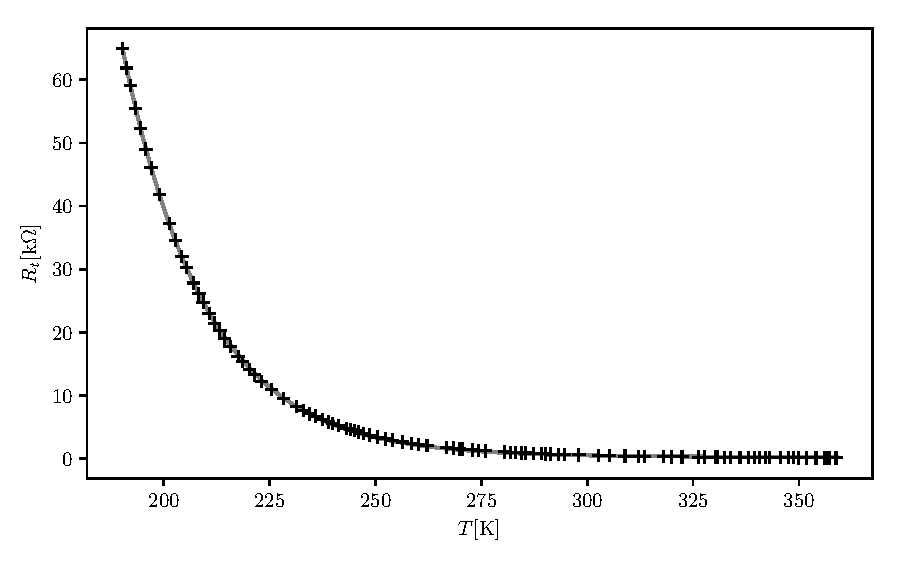
\includegraphics[]{rt}
\caption{Závislost odporu termistoru na teplotě}
\label{fig:rt}
\end{figure}

\subsection*{Úkol 3 a 4}

V grafu \ref{fig:fit_log_R} je zobrazena lineární závislost $\log R_t$ na $1/T$ spolu s regresní přímkou podle rovnice \eqref{eq:log_R}. Z té jsme určili hodnoty
$$ B = \SI{2610 \pm 12}{\kelvin}, $$
$$ R_\infty = \SI{0.086 \pm 0.004}{\ohm}. $$
Podle vzorce \eqref{eq:delta_U} byla spočtena aktivační energie $\Delta U$ a podle \eqref{eq:alpha} teplotní součinitel odporu při teplotě $\SI{298.15}{\kelvin}$
$$ \Delta U = \SI{43.40 \pm 0.19 e3}{\joule\per\mole}, $$
$$ \alpha = \SI{29.4 \pm 0.2 e-3}{\per\kelvin}. $$

Graf \ref{fig:va} ukazuje statickou voltampérovou charakteristiku termistoru a teplotu termistoru při protékajícím proudu, vypočtenou podle \eqref{eq:K}. Potřebné konstanty $T_0$ a $T_m$ byly určeny z lineární regrese lineární části grafu \ref{fig:va} a srovnáním s průběhem teplotní závislosti odporu, respektive ze vztahu \eqref{eq:teplota_v_max}:
$$ T_0 = \SI{295.5 \pm 0.5}{\kelvin},$$
$$ T_m = \SI{339.7 \pm 0.7}{\kelvin}. $$

Konstanta $K$ byla spočtena podle vzorce \eqref{eq:K} s použitím výše uvedených konstant
$$ K = \SI{7.14 \pm 0.08 e3}{\kelvin\per\watt}. $$
\begin{figure}[H]
\centering
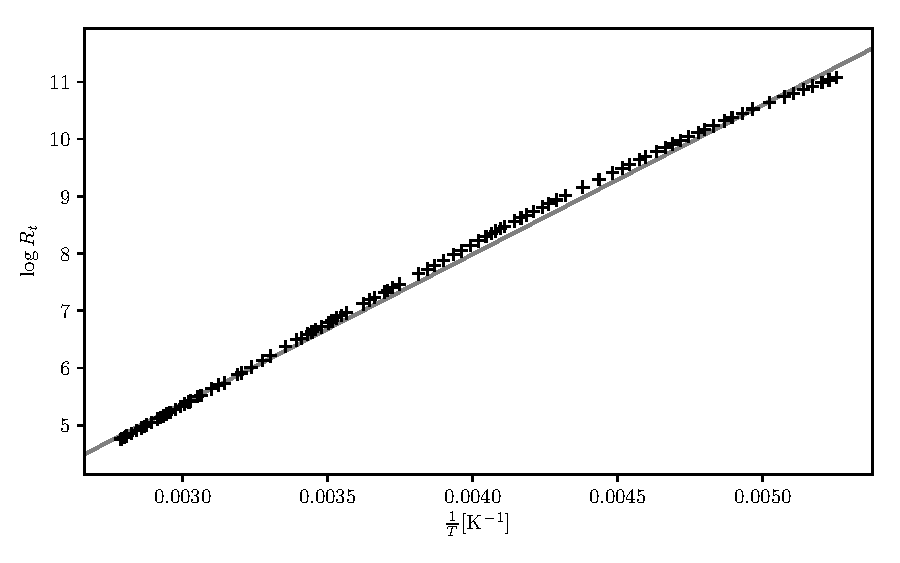
\includegraphics[]{fit_log_R}
\caption{Lineární regrese závislosti $\log R_t$ na $1/T$}
\label{fig:fit_log_R}
\end{figure}

\begin{figure}[H]
\centering
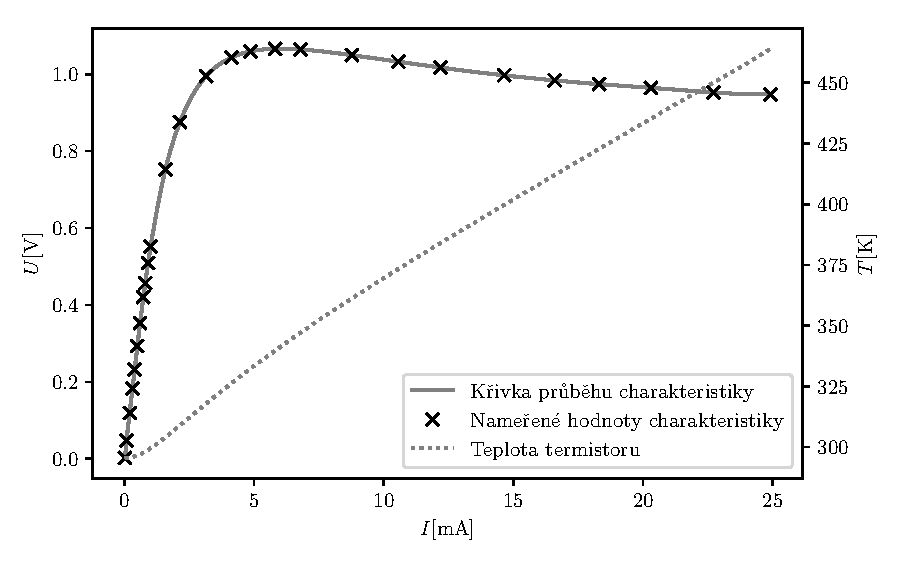
\includegraphics[]{va}
\caption{Statická voltampérová charakteristika termistoru s průběhem teploty}
\label{fig:va}
\end{figure}



\end{document}
